\documentclass[10pt]{beamer}
\usetheme[
%%% options passed to the outer theme
%    progressstyle=movCircCnt,   %either fixedCircCnt, movCircCnt, or corner
%    rotationcw,          % change the rotation direction from counter-clockwise to clockwise
%    shownavsym          % show the navigation symbols
  ]{AAUsimple}
  
% If you want to change the colors of the various elements in the theme, edit and uncomment the following lines
% Change the bar and sidebar colors:
%\setbeamercolor{AAUsimple}{fg=red!20,bg=red}
%\setbeamercolor{sidebar}{bg=red!20}
% Change the color of the structural elements:
%\setbeamercolor{structure}{fg=red}
% Change the frame title text color:
%\setbeamercolor{frametitle}{fg=blue}
% Change the normal text color background:
%\setbeamercolor{normal text}{fg=black,bg=gray!10}
% ... and you can of course change a lot more - see the beamer user manual.

\usepackage[utf8]{inputenc}
\usepackage[english]{babel}
\usepackage[T1]{fontenc}
% Or whatever. Note that the encoding and the font should match. If T1
% does not look nice, try deleting the line with the fontenc.
\usepackage{helvet}

% colored hyperlinks
\newcommand{\chref}[2]{%
  \href{#1}{{\usebeamercolor[bg]{AAUsimple}#2}}%
}

\title{Private memoirs of a smart meter}

\subtitle{Andrés Molina-Markham, Prashant Shenoy, Kevin Fu, Emmanuel Cecchet, David Irwin}  % could also be a conference name

\date{\today}

\author{
  Bruno Thalmann\\
  \href{mailto:bthalm11@student.aau.dk}{{\tt bthalm11@student.aau.dk}}
}

% - Give the names in the same order as they appear in the paper.
% - Use the \inst{?} command only if the authors have different
%   affiliation. See the beamer manual for an example

\institute[
%  {\includegraphics[scale=0.2]{aau_segl}}\\ %insert a company, department or university logo
  Dept.\ of Computer Science\\
  Aalborg University\\
  Denmark
] % optional - is placed in the bottom of the sidebar on every slide
{% is placed on the bottom of the title page
  Department of Computer Science\\
  Aalborg University\\
  Denmark
  
  %there must be an empty line above this line - otherwise some unwanted space is added between the university and the country (I do not know why;( )
}

% specify a logo on the titlepage (you can specify additional logos an include them in 
% institute command below
\pgfdeclareimage[height=1.5cm]{titlepagelogo}{AAUgraphics/aau_logo_new} % placed on the title page
%\pgfdeclareimage[height=1.5cm]{titlepagelogo2}{AAUgraphics/aau_logo_new} % placed on the title page
\titlegraphic{% is placed on the bottom of the title page
  \pgfuseimage{titlepagelogo}
%  \hspace{1cm}\pgfuseimage{titlepagelogo2}
}

\begin{document}
% the titlepage
{\aauwavesbg%
\begin{frame}[plain,noframenumbering] % the plain option removes the header from the title page
  \titlepage
\end{frame}}
%%%%%%%%%%%%%%%%

% TOC
\begin{frame}{Agenda}{}
\tableofcontents
\end{frame}
%%%%%%%%%%%%%%%%

\section{Privacy Concerns}
\begin{frame}{A list of concerns}{}
\end{frame}

\section{Monitored smart meter example}
\begin{frame}{Setup}
  \begin{itemize}
    \itemsep2em 
    \item 60 days of power consumption
    \item 3 homes
    \item Power activity journals(min. 3 days)
    \item TED energy monitor
    \end{itemize}
\end{frame}

\begin{frame}{Setup}
  \begin{center}
  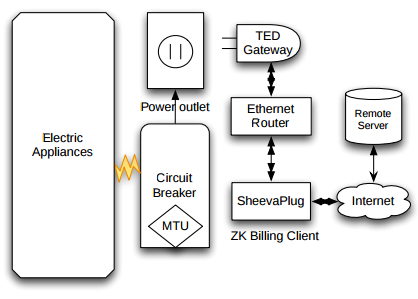
\includegraphics[scale=.5]{graphics/TED_architecture.png}  
  \end{center}
  \begin{itemize}
  \item Outputs: $(t,p)$ for each second
  \end{itemize}
\end{frame}

\begin{frame}{Analysis}
  \begin{enumerate}
    \itemsep2em 
  \item Pre-process data using clustering alogrithm
  \item Tag power events with their characteristics
  \item Filter out automated appliances
  \item Map opaque labels to real-life events from external data
  \end{enumerate}
\end{frame}

\begin{frame}{Pro-process}
  Output: power segments
\end{frame}

\begin{frame}{Tag events}
  \begin{itemize}
  \item Each power segments gets labeled
  \item 6 tuple: (segment label, start time, average power, duration, beginning power step, shape label)
  \item Answer questions
  \end{itemize}
\end{frame}
%%%%%%%%%%%%%%%%

\section{Privacy enhancing smart meter architecture}
\begin{frame}{Components}
  \begin{itemize}
  \item Smart meter
  \item Neighborhood gateways
  \item Remote server
  \end{itemize}
  
\end{frame}

{\aauwavesbg
\begin{frame}[plain,noframenumbering]
  \finalpage{Questions}
\end{frame}}
%%%%%%%%%%%%%%%%

\end{document}
